\lecture{3}{3. Februar 2025}{Crystalline solids}

\section{Crystalline solids}

\subsection{Atomic arrangements and packing}
\begin{figure} [ht]
  \centering
  \caption{Atomic bonding energy as a function of bonding length}
  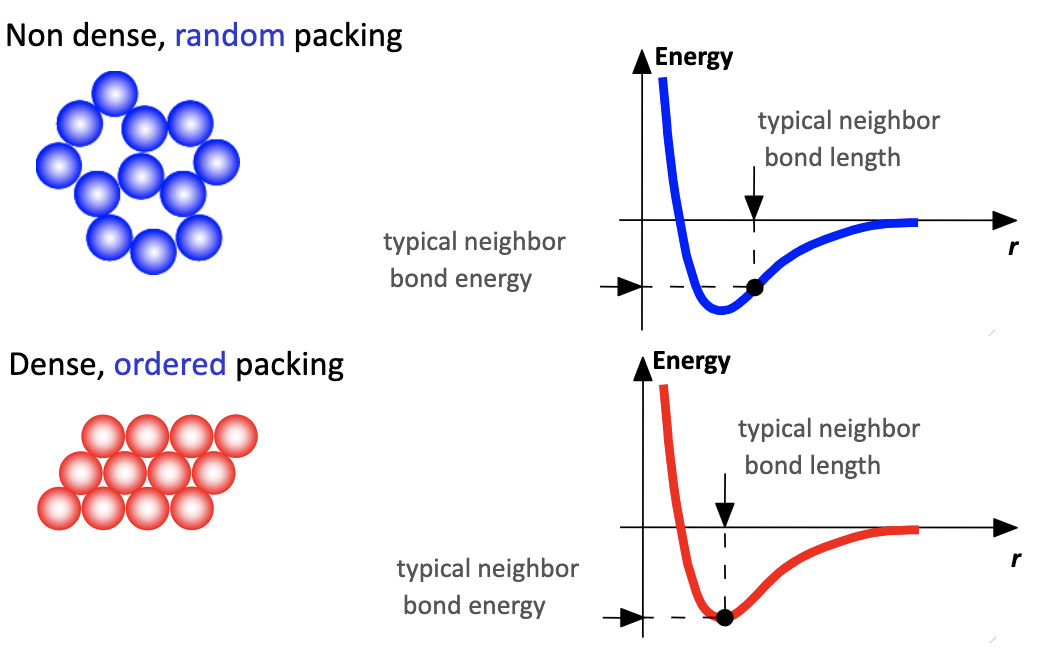
\includegraphics[width=0.5\linewidth]{./figures/f3_1.png}
  \label{fig:f3_1}
\end{figure}
As everything else, atoms tend to organize themselves in a manner that minimizes the energy -- in the case of atoms the energy in question is bonding energy. As we learned last week bonding energy is a function of length and thus the atoms will tend to keep some ``optimal'' distance between themselves. This leads to orderly packing. An atomic structure with long-range periodicity is called \textit{crystalline} and an atomic structure without this periodicity is called \textit{noncrystalline} or \textit{amorphous}. Most noncrystalline materials are formed as a result of rapid cooling. This is shown in \textbf{\autoref{fig:f3_1}}.

\begin{definition}[Crystalline]
  ``A \textit{crystalline} material is one in which the atoms are situated in a repeating or periodic array over large atomic distances -- that is, long range order exists, such that upon solidification, the atoms will position themselves in a repetitive three-dimensional pattern, in which each atom is bonded to its nearest neighbor atom.''
\end{definition}

\begin{definition}[Crystal structure]
  ``A \textit{crystal structure} is the manner in which atoms, ions, or molecules are spatially arranged.''
\end{definition}

\begin{definition}[Lattice]
  ``A \textit{lattice} means a three-dimensional array of points coinciding with atom positions (or sphere centers)''
\end{definition}

\subsection{Unit cell}
\begin{figure} [ht]
  \centering
  \caption{The two representations of unit cells.}
  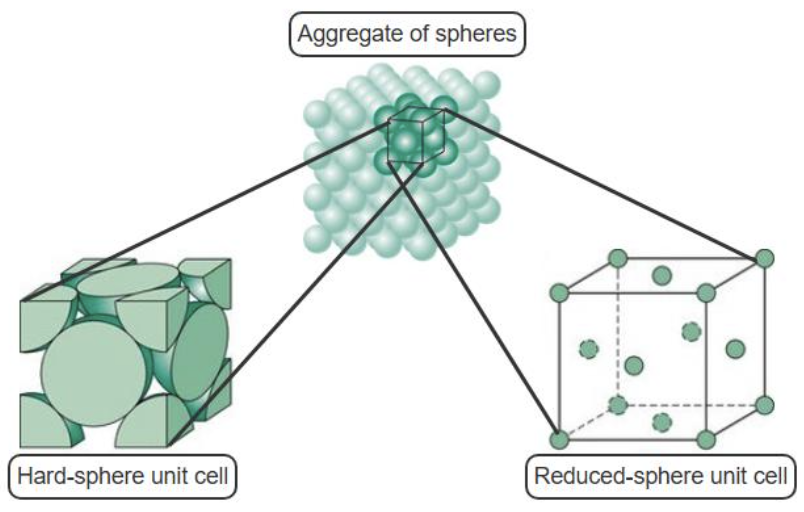
\includegraphics[width=0.5\linewidth]{./figures/f3_2.png}
  \label{fig:f3_2}
\end{figure}
\begin{definition}[Unit cell]
  A unit cell is the most basic structural building block of a material. The unit cell completely defines the materials structure based on its geometry. For some materials multiple unit cells can be chosen but we usually choose the unit cell with the highest level of geometrical symmetry. These are typically shown either with the ``hard sphere model'' or with the ``reduced sphere model'' as shown in \textbf{\autoref{fig:f3_2}}.
\end{definition}

\subsection{Crystal structures for metals}
Most metals have 1 of 3 different crystal structures. These are
\begin{itemize}
  \item Face-centered cubic (FCC)
  \item Body-centered cubic (BCC)
  \item Hexagonal close-packed (HCP)
\end{itemize}
\begin{figure} [ht]
  \centering
  \caption{Examples of common crystal structures for metals.}
  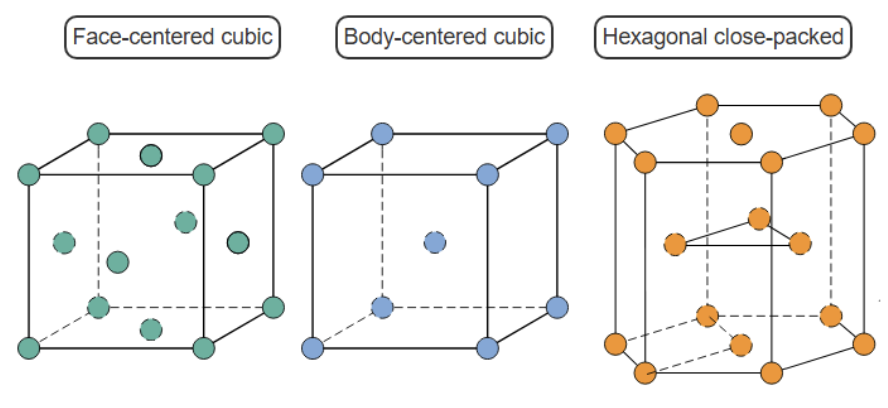
\includegraphics[width=0.5\linewidth]{./figures/f3_3.png}
  \label{fig:f3_3}
\end{figure}
These common metallic crystal structures are shown in \textbf{\autoref{fig:f3_3}}. In \textbf{\autoref{fig:f3_4}} a table of metals and their corresponding crystal structure is shown.
\begin{figure} [ht]
  \centering
  \caption{Metals and their crystal structure.}
  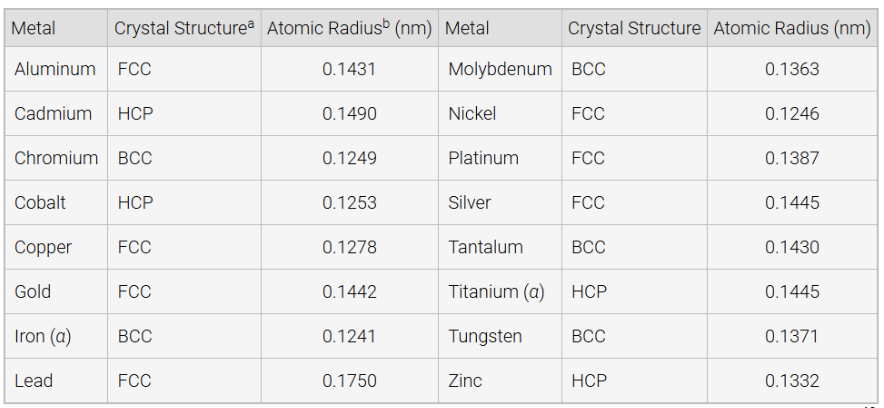
\includegraphics[width=0.5\linewidth]{./figures/f3_4.png}
  \label{fig:f3_4}
\end{figure}

\subsection{Atomic packing factor}
To calculate the number of atoms within a unit cell $N$ one can use the formula
\[ 
N = N_i + \frac{N_f}{2} + \frac{N_c}{8}
.\]
Where $N_i$ is the number of interior atoms, $N_f$ is the number of face atoms and $N_c$ is the number of corner atoms.

The atomic packing factor (APF) can then be calculated as
\[ 
\mathrm{APF} = \frac{\text{volume of atoms in unit cell (hard spheres)}}{\text{Volume of unit cell}}
.\]
Another related concept is that of the \textit{coordination number}.
\begin{definition}[Coordination number]
  The coordination number is the number of atoms that ``touches'' any given atom in the unit cell. That is the amount of atoms sharing the smallest distance to a given atom.
\end{definition}

\subsection{Theoretical density of a material}
The theoretical density of a material can be calculates solely based on the geometry of the unit cell and chemical mmaterial-specific values. The formula is
\[ 
\rho = \frac{\text{Mass of atoms in UC}}{\text{Volume of UC}} = \frac{nA}{V_c N_a}
.\]
Where $n$ is the number of atoms per unit cell, $A$ is the atomic weight, $V_c$ is the volume of the unit cell and $N_a$ is avogadros constant.

\subsection{Crystal systems}
Any crystal structure can be described based on 6 parameters relating to the unit cells. These are called the \textit{lattice parameters} and consist of edge lengths and interaxial angles. 

\begin{definition}[Crystal systems]
  A \textit{crystal system} is a scheme in which crystal structures are classified based on the geometry of the UC. This geometry is specified in terms of the \textit{lattice parameters}. The 7 different crystal systems are shown in \textbf{\autoref{fig:f3_5}}.
\end{definition}
\begin{figure} [ht]
  \centering
  \caption{The 7 different crystal systems and their axial relationships and interaxial angles.}
  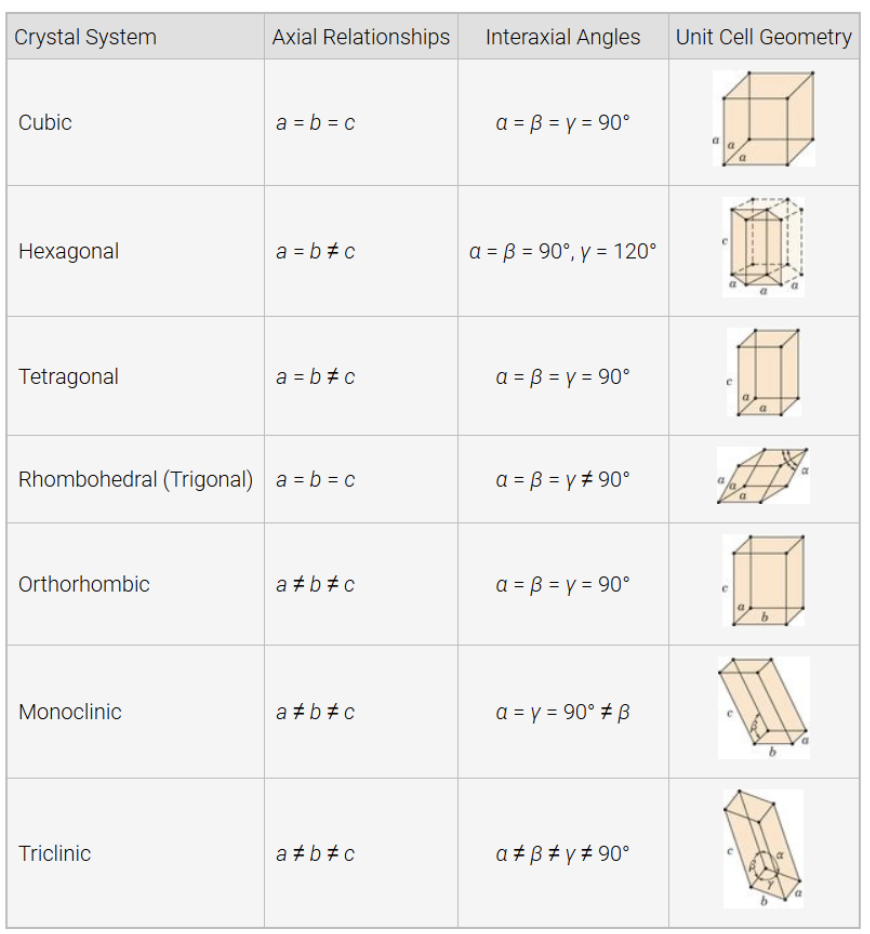
\includegraphics[width=0.5\linewidth]{./figures/f3_5.png}
  \label{fig:f3_5}
\end{figure}

\subsection{Point coordinates}
For a general cubic structure there are three different specific edge-lengths. Any position within the UC can be represented by a so-called \textit{point coordinate}. Point coordinates are given as a \textit{fractional multiple} of $a$, $b$, and $c$ -- the edge lengths of the UC. A Point coordinate is given as a list of the fractional multiples without commas. That is for the outer upper corner -- which is placed at $1$ on both the $a$, $b$, and $c$-axis we get a point coordinate of 111 (1, 1, 1 -- but without commas). The general algorithm is:
\begin{itemize}
  \item Determine your lattice position (for outer upper corner this is 1, 1, 1.)
  \item Divide by edge lengths of UC
\[ 
\frac{a}{a} \frac{b}{b} \frac{c}{c} = 1 1 1
.\]
  \item Concatenate the numbers to get 111
\end{itemize}

\subsection{Crystallographic direcions}
Not just positions in the UC can be represented numerically. The same is true for directions. The general algorithm for this is
\begin{itemize}
  \item Determine the coordinates of the vector tail $p_1$ and vector head $p_2$.
  \item Subtract tail coordinates from head coordinates.
  \item Normalize coordinate differences in terms of lattice parameters $a$, $b$, and $c$. (Divide by $a$, $b$, and $c$).
  \item Reduce to smallest integer values.
  \item Enclose indices in square brackets without commas like $[uvw]$.
  \item Note: Negative values are written as $\overline{x}$ where $\overline{x} = -x$.
\end{itemize}

\begin{exa}[Crystallographic direction]
  We want to determine the crystallographic direction from pt. 1: $x_1 = 0, y_1 = 0, z_1 = 0$ to pt. 2: $x_2 = a, y_2 = 0, z_2 = \frac{c}{2}$.
  \bigbreak
  Firstly we get the three indices as
  \begin{align*}
    \Delta x &= 1\\
    \Delta y &= 0 \\
    \Delta z &= \frac{1}{2}
  .\end{align*}
  This gives $[1, 0, \frac{1}{2}]$. This is then reduced to integer values as $[2, 0, 1]$. Commas can now be removed and we get $[201]$. If the $z$-direction had been negative the crystallographic direction would instead be $\left[ 2 0 \overline{1} \right]$.
\end{exa}

\begin{definition}[Linear density of atoms]
  The \textit{linear density of atoms} is defined as the number of atoms \textit{centered} on a direction vector divided by the length of the direction vector.
\end{definition}

\subsection{Crystallographic planes}
Parallel to the notion of crystallographic points and crystallographic direction is \textit{crystallographic planes}. These are defined in terms of the so-called \textit{miller-indices} of the plane. The general algorithm for this is
\begin{itemize}
  \item Choose an origin and a plane.
  \item If the chosen plane passes through the origin choose a new plane or a new origin.
  \item Read of the values of intercept with the $x$, $y$ and $z$ axes in terms of $a$, $b$, and $c$.
  \item Take the reciprocals of the intercepts.
  \item Normalize the reciprocals of intercepts by multiplying by lattice parameters $a$, $b$ and $c$.
  \item Reduce to smallest integer values.
  \item Enclose the resulting \textit{miller indices} in parenthesis with no commas like $(hkl)$. If any values are negative these can be shown as $\overline{x}$ where $\overline{x} = x$
\end{itemize}
Examples of this algorithm are shown in \textbf{\autoref{fig:f3_6}}, \textbf{\autoref{fig:f3_7}} and \textbf{\autoref{fig:f3_8}}.
\begin{figure}[ht]
  \centering
  % First figure
  \begin{minipage}[t]{0.32\textwidth}
    \centering
    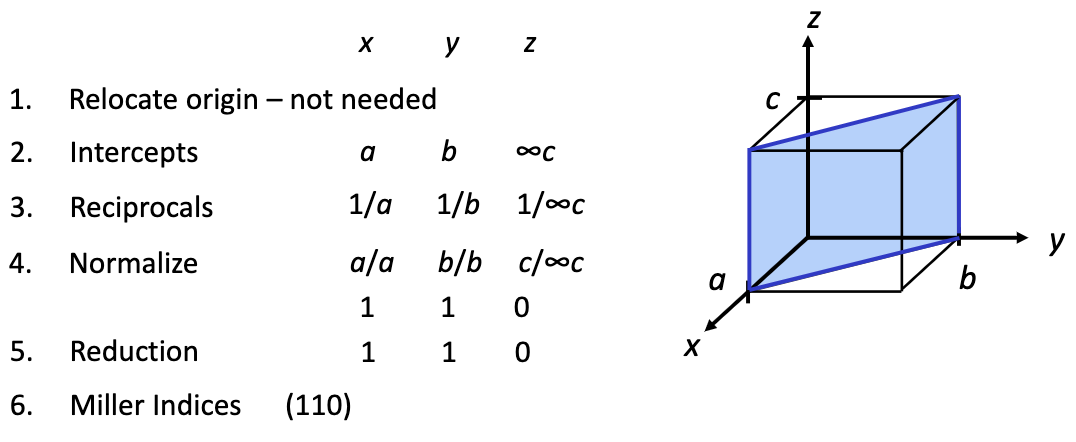
\includegraphics[width=\linewidth]{./figures/f3_6.png}
    \caption{Example 1 of a crystallographic plane.}
    \label{fig:f3_6}
  \end{minipage}%
  \hfill
  % Second figure
  \begin{minipage}[t]{0.32\textwidth}
    \centering
    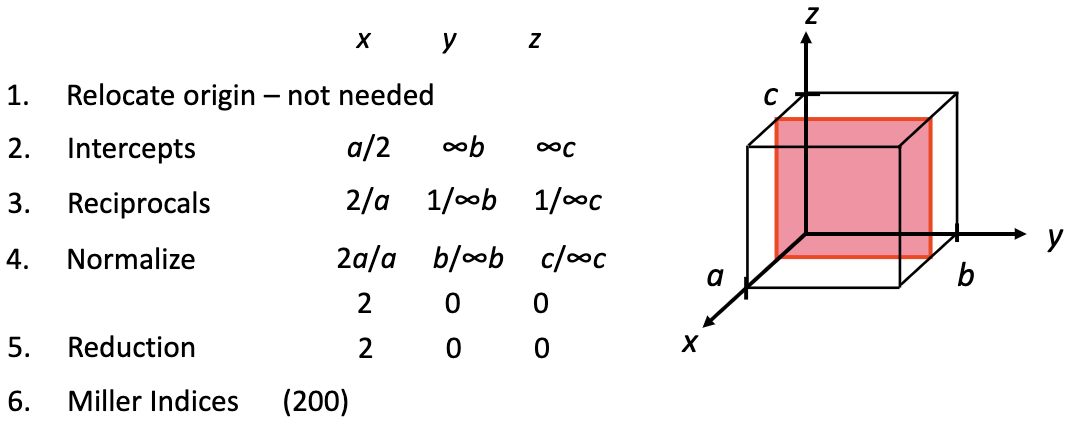
\includegraphics[width=\linewidth]{./figures/f3_7.png}
    \caption{Example 2 of a crystallographic plane.}
    \label{fig:f3_7}
  \end{minipage}%
  \hfill
  % Third figure
  \begin{minipage}[t]{0.32\textwidth}
    \centering
    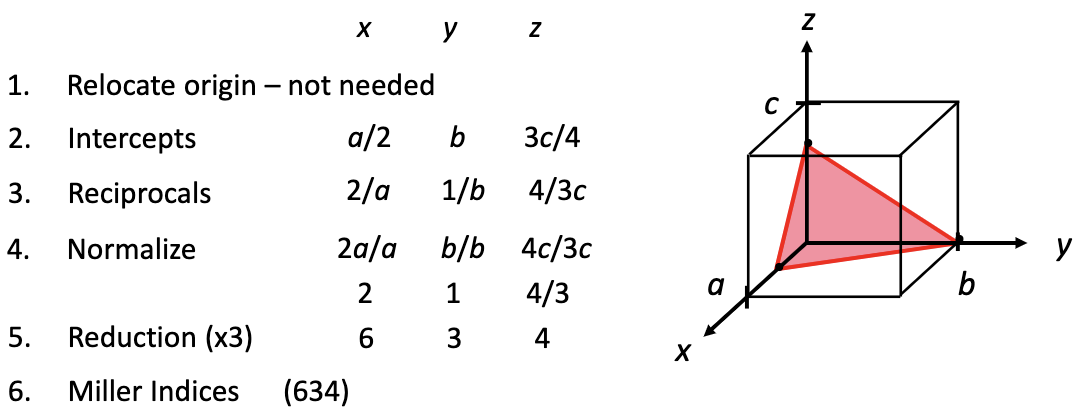
\includegraphics[width=\linewidth]{./figures/f3_8.png}
    \caption{Example 3 of a crystallographic plane.}
    \label{fig:f3_8}
  \end{minipage}
\end{figure}

\begin{definition}[Planar density of atoms]
  As was the case for the linear density a planar density of atoms can also be defined. This is defined as the number of atoms centered on a plane divided by the area of the plane. 
\end{definition}
